\entry{2026-10-20}{Priority 4: robustness --- random rules, retraining seeds, hardware}

Lane \texttt{2026-10-19-jcp-robust}, last commit \texttt{cbf574373}, mirror \texttt{d49bd0085}. A100/H200 jobs (\texttt{jax\_backend=gpu}), 46.4 of 95 GPU-h; every results audit accepted, report audit 3 ACCEPT. Numbers quoted from the generated \path{report.md}; errors E0-conditional.

\begin{itemize}
\item \textbf{E1 random quadrature draws (16 each):} in 3D both registered configurations are robust and insensitive (the deployed W512 draw is the least favourable of 16 but still qualifies). In 2D the R128 BE arms at $2\Delta t_0$ and $2.5\Delta t_0$ are ``fragile'' at all meshes --- but every failing draw fails only on distance to its own successor rule; all stay within $2.02\times10^{-4}$ of the independent target, and accuracy is insensitive in every cell.
\item \textbf{E2 full retraining, seeds 1--3:} in 2D, 140 of 183 verdict rows are seed-robust, 21 seed-dependent, 22 inconclusive. \textbf{Mesh-independence of accuracy and the improvement with $r$ survive retraining.} The selected quadrature rule changes with the seed, and the deployed R128 rule fails qualification on all three retrained banks (R384 on two) --- rule selection is a per-bank step. In 3D (129 rows: 45/17/67), accuracy improves with width on every seed for the fixed Gauss rule; worst-case error at W1024 varies up to 1.9$\times$ across seeds (median 1.009$\times$); W768--W1024 have almost no certified rules. Coordinator recount of the verdict files: identical counts.
\item \textbf{E5 hardware (A100 vs H200, two jobs each):} 5 of 6 registered verdicts agree, 1 inconclusive, none contradicts; 4 of 10 cost ratios are hardware-dependent.
\end{itemize}
\begin{center}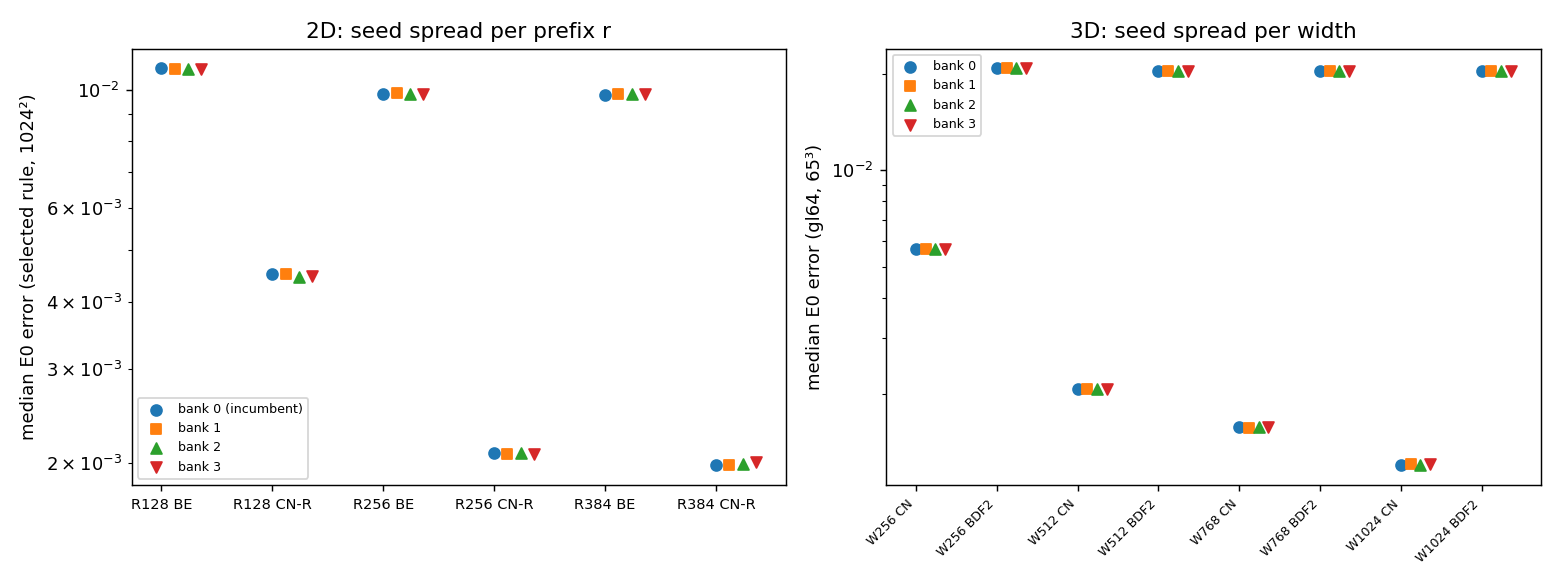
\includegraphics[width=0.48\linewidth]{figs/rb_e2_spread.png}\hfill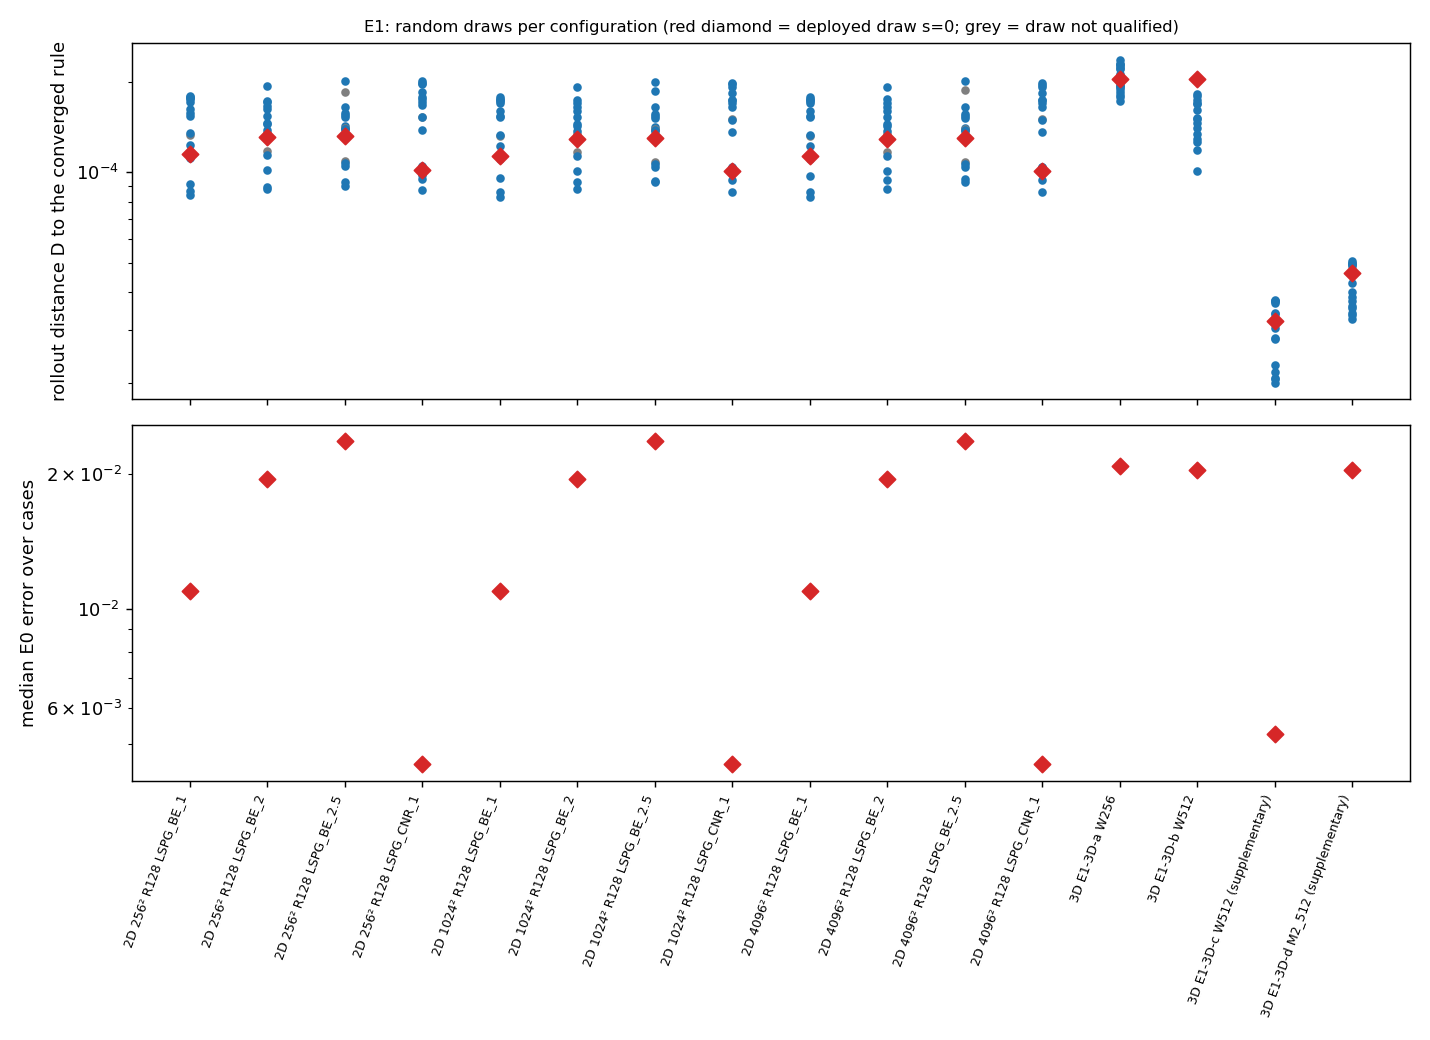
\includegraphics[width=0.48\linewidth]{figs/rb_e1_draws.png}\end{center}
\subsection*{Corrections}
\retracted{The first E2 2D roll-up used the wrong dominance rule; its counts (107/18/22) and the claim that R256 front membership is seed-dependent are withdrawn (A17). Report-generation errors (double-counted GPU-hours, a statement contradicting the verdict table, wrong glossary definitions, a misread data hash) were fixed (A19--A21). One job timed out and one was cancelled after under-estimated certificates.}
